\documentclass[paper]{aiaaNew}
% cover, paper, article, note,submit

%\usepackage[notref,notcite]{showkeys}


\newenvironment{proof}
{}{}


%\documentstyle[10pt,draft,fancyheadings]{AIAAtran}
%\documentstyle[9pt,twocolumn,technote,twoside]{AIAAtran}


\SubmitName{Schaub}

% for conference paper:
\usepackage{AVS}
\usepackage{amsmath,amsfonts,amssymb}
\usepackage{subfigure}
\usepackage{multirow}
\usepackage{float}

\newcommand{\specialcell}[2][c]{%
  \begin{tabular}[#1]{@{}c@{}}#2\end{tabular}}

\PaperNumber{xxx}

\CoverFigure{}

\Conference{{\bfseries AIAA Guidance, Navigation and \\ Control 
		Conference} \\
	August 10--12,~1998 / Boston, MA}

% for a journal simulation cover page:

\JournalName{Journal of Guidance, Navigation and Control}
\JournalIssue{Volume~xx, Number~xx, Jan.--Feb., 2001, Pages xx--xx}

% journal article simulation:

\ArticleIssue{Vol.~24, No.~1, Jan.--Feb., 2001}% first page
\ArticleHeader{Schaub Et Al: New Penalty Functions}% subsequent pages

% journal note simulation:

\NoteHeader{J.Guidance, Vol.~20, No.~13: Engineering Notes}

% set copyright and other notices to appear
% as a footnote at the bottom of the first page:

%\PaperNotice{\CopyrightB{1998}{Hanspeter Schaub}}

\JournalNotice{Presented as Paper~06--3792 at the AIAA
	Guidance, Navigation and Control Conference, San 
	Diego,~CA,
	July~29--31,~1996.
	\CopyrightB{1996}{the authors}}

% load the title, author, and abstract for use with the \maketitle command

\title{Derivation of EOMs for $N_p+1$ Connected Panels using Kane's Method}
%\author{Iosto Fodde}
\begin{document}
	
	
	\maketitle

\section{Introduction}
$\theta_i = \theta_{i,d} + \theta_{i,0}$ positive angle is in the upward direction.
\begin{figure}[H]
    \centering
    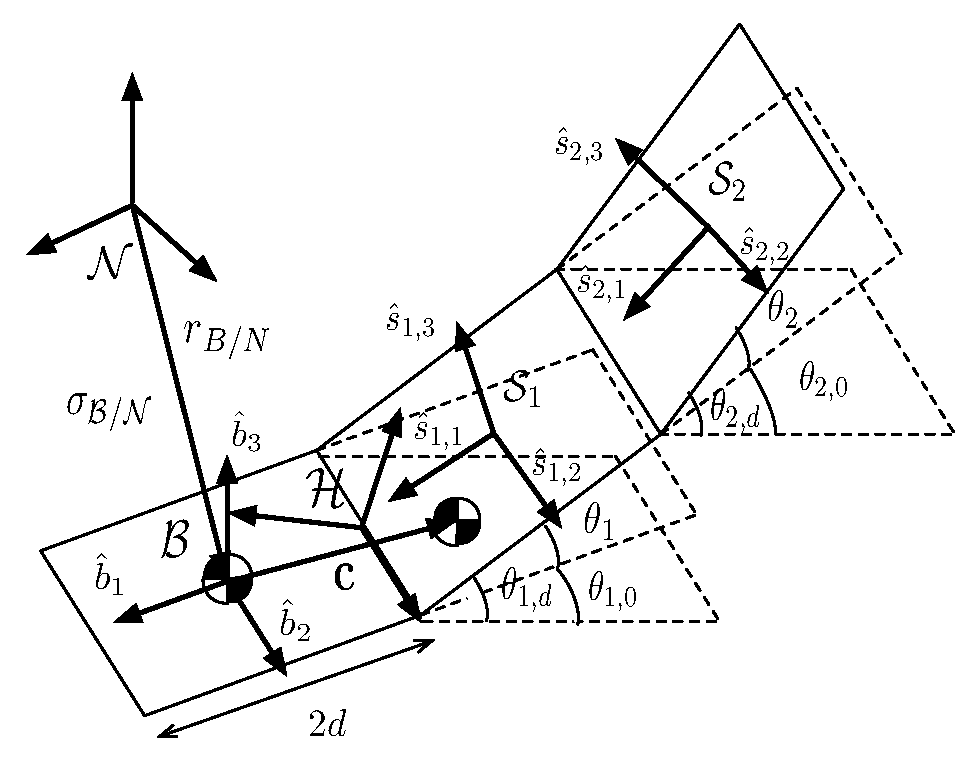
\includegraphics[scale=0.5]{Figures/conn_panels5.pdf}
    \label{fig:system}
    \caption{Frame and variable definitions for the system discussed here, where $N_p=2$.}
\end{figure}
\section{Derivation of Equations of Motion - Kane's Method}
	
The choice of state variables and their respective chosen generalized speeds are:
	
\begin{equation}
	\bm X = 
	\begin{bmatrix}
	\bm r_{B/N}\\
	\bm \sigma_{\cal{B/N}}\\
	\theta_1\\
	\cdot\\
	\theta_{N_p}
	\end{bmatrix}
	\quad
	\bm u = \begin{bmatrix}
	\dot{\bm r}_{B/N}\\
	\bm \omega_{\cal{B/N}}\\
	\dot{\theta}_1\\
	\cdot\\
	\dot{\theta}_{N_p}
	\end{bmatrix}
\end{equation} 	
To create the partial velocity table, some velocities first need to be defined

\begin{equation}
\dot{\bm r}_{B/N} = \dot{\bm r}_{B/N}
\end{equation}

\begin{equation}
\dot{\bm r}_{C/N} = \dot{\bm r}_{B/N} + \dot{\bm c}
\label{eq:rDot_CN}
\end{equation}

\begin{equation}
\bm \omega_{\cal{B/N}} = \bm \omega_{\cal{B/N}}
\end{equation}

\begin{equation}
\bm \omega_{\cal S_{\textit{i}/N}} = \bm \omega_{\cal{B/N}} + \Big(\sum_{k=1}^{i} \dot{\theta}_k \Big) \bm{\hat{s}}_{i,2}
\end{equation}

\begin{equation}
\label{eq:rsin}
\bm r_{S_{i}/N} = \bm r_{B/N} + \bm r_{S_{i}/B} = \bm r_{B/N} + \bm r_{H/B} - [d\bm{\hat{s}}_{i,1} + \sum_{n=1}^{i-1} 2d\bm{\hat{s}}_{n,1} ]
\end{equation}

\begin{equation}
\label{eq:rsindot}
\dot{\bm r}_{S_{i}/N} = \dot{\bm r}_{B/N} + {\bm r}'_{S_{i}/B} + \bm \omega_{\cal{B/N}} \times {\bm r}_{S_{i}/B} = \dot{\bm r}_{B/N} + d\Big[\Big(\sum_{k=1}^{i} \dot{\theta}_k \Big) \bm{\hat{s}}_{i,3} + \sum_{n=1}^{i-1} 2\bm{\hat{s}}_{n,3}\Big(\sum_{k=1}^{n} \dot{\theta}_k \Big) \Big]  - [\tilde{{\bm r}}_{S_{i}/B}] \bm \omega_{\cal{B/N}}
\end{equation}
Where
\begin{equation}
\label{eq:sijp}
\hat{\bm s}'_{i,j} = \bm\omega_{\cal{S}_{\textit{i}}/\cal{B}}\times\hat{\bm s}_{i,j}=\Big(\sum_{k=1}^{i} \dot{\theta}_k \Big)\hat{\bm s}_{i,2}\times\hat{\bm s}_{i,j}
\end{equation}
is used to get the derivative.\\
The summation in equation \ref{eq:rsin} and \ref{eq:rsindot} can be out of bounds for certain values of $i$. When this occurs, the summation becomes equal to zero. $\bm c$ is defined as the position vector between the body frame and the COM of the system:
\begin{equation}
    \bm c = \frac{1}{m_{sc}}\Big[ \sum_{i=1}^{N_p} m_p {\bm r}_{S_i/B}\Big]
\end{equation}
\begin{equation}
\dot{\bm c} = {\bm c}' - [\tilde{\bm c}]{\bm \omega}_{\cal{B/N}} 
\end{equation}
\begin{equation}
{\bm c}' = \frac{m_p d}{m_{sc}} \sum_{i=1}^{N_p} \Big[\Big(\sum_{k=1}^{i} \dot{\theta}_k \Big) \bm{\hat{s}}_{i,3} + \sum_{n=1}^{i-1} 2\bm{\hat{s}}_{n,3}\Big(\sum_{k=1}^{n} \dot{\theta}_k \Big) \Big] 
\label{eq:cprime1}
\end{equation}
\begin{equation}
{\bm c}' = \frac{m_p d}{m_{sc}} \Big[\sum_{i=1}^{N_p} \dot{\theta}_i  \sum_{n=i}^{N_p} (2[N_p - n]+1 )\bm{\hat{s}}_{n,3}\Big] 
\label{eq:cprime2}
\end{equation}
Now the following partial velocity table can be created (here: $j = r-6$):

\begin{table}[H]
	\caption{Partial Velocity Table}
	\label{tab:hub}
	\centering \fontsize{10}{10}\selectfont
	\begin{tabular}{ |c | c | c | c | c | c |} % Column formatting, 
		\hline
		$r$ & $\bm v^{C}_{r}$ & $\bm v^{B}_{r}$  & $\bm \omega_{\textit{r}}^{\cal{B}}$ & $\bm v^{S_i}_{r}$ & $\bm \omega_{\textit{r}}^{\cal{S}_\textit{i}}$ \\
		\hline \hline
		$1-3$ & $[I_{3\times 3}]$ & $[I_{3\times 3}]$ & $[0_{3\times 3}]$ & $ [I_{3\times 3}]$ & $[0_{3\times 3}]$ \\ \hline
		$4-6$ & $-[\tilde{\bm c}]$ & $[0_{3\times 3}]$ & $[I_{3\times 3}]$ & $ - [\tilde{{\bm r}}_{S_{i}/B}]$ & $[I_{3\times 3}]$ \\ \hline
		$7-{N_p}$ & $\sum_{n=j}^{N_p} (2[N_p - n]+1 )\bm{\hat{s}}_{n,3} $ & $[0_{3\times 1}]$ & $[0_{3\times 1}]$ & \specialcell{if $j \leq i$ : \\ $d [\bm{\hat{s}}_{i,3} + \sum^{i-1}_{n=j} 2\bm{\hat{s}}_{n,3}] $ \\ else:\\ $[0_{3\times 1}]$\\  }& \specialcell{if $j \leq i$ : \\ $\bm{\hat{s}}_{i,2} $ \\ else:\\ $[0_{3\times 1}]$} \\
		\hline
	\end{tabular}
\end{table}
Using these partial velocity definitions, the follow sections will step through the formulation for the translational, rotational and panel EOMs developed using Kane's method.

\subsection{Hub Translational Motion}
Starting with the definition of a generalized force:

\begin{equation}
\bm F_r = \sum\limits_{r}^{N} \bm v_r^T \bm F
\label{eq:genActive}
\end{equation}
Using this definition the external force applied on the system for the translational equations is defined as:

\begin{equation}
\bm F_{1-3} = [\bm v^C_{1-3}]^T \bm F_{\text{ext}} = \bm F_{\text{ext}}
\end{equation}
Using the definition of generalized inertia forces,
\begin{equation}
\bm F^*_r = \sum\limits_{r}^{N}\Big[\bm \omega_r^T \bm T^* +  \bm v_r^T (- m_r \bm a_r)\Big]
\label{eq:genInert}
\end{equation}
the inertia forces for the hub translational motion are defined as
	
\begin{equation}
\bm F^*_{1-3} = [\bm v^{B}_{1-3}]^T (-m_{\text{hub}} \ddot{\bm r}_{B/N}) + \sum\limits_{i=1}^{N_p}[\bm v^{S_i}_{1-3}]^T (-m_{\text{p}_i} \ddot{\bm r}_{S_{i}/N}) = -m_{\text{hub}} \ddot{\bm r}_{B/N} + \sum\limits_{i=1}^{N_p} -m_{\text{p}_i}\ddot{\bm r}_{S_{i}/N}
\end{equation}

Finally, Kane's equation is:

\begin{equation}
\bm F_r + \bm F^*_r = 0
\label{eq:KanesEq}
\end{equation}
therefore
\begin{equation}
\bm F_{\text{ext}} -m_{\text{hub}} \ddot{\bm r}_{B/N} + \sum\limits_{i=1}^{N_p} -m_{\text{p}_i}\ddot{\bm r}_{S_{i}/N} = 0
\end{equation}
Expanding and rearranging results in
\begin{equation}
m_{\text{hub}} \ddot{\bm r}_{B/N}  + \sum\limits_{i=1}^{N_p} m_{\text{p}} (\ddot{\bm r}_{B/N} + \ddot{\bm r}_{S_{i}/B}) = \bm F_{\text{ext}}
\label{eq:KanesTrans}
\end{equation}
Where
\begin{equation}
\ddot{\bm r}_{S_i/B} = \bm{r}''_{S_i/B} + 2 \bm\omega_{\cal B/N} \times \bm{r}'_{S_i/B} +  \dot{\bm\omega}_{\cal B/N} \times \bm{r}_{S_i/B} + \bm\omega_{\cal B/N} \times (\bm\omega_{\cal B/N} \times \bm{r}_{S_i/B})
\label{eq:rsddot}
\end{equation}
Plugging Eq.~\eqref{eq:rsddot} into Eq.~\eqref{eq:KanesTrans} results in
\begin{multline}
m_{\text{hub}} \ddot{\bm r}_{B/N} +  \sum\limits_{i=1}^{N_p} m_{\text{p}} \Big[\ddot{\bm r}_{B/N} +  \bm{r}''_{S_i/B}
+ 2 \bm\omega_{\cal B/N} \times \bm{r}'_{S_i/B} +  \dot{\bm\omega}_{\cal B/N} \times \bm{r}_{S_i/B}
\\ + \bm\omega_{\cal B/N} \times (\bm\omega_{\cal B/N} \times \bm{r}_{S_i/B})\Big] = \bm F_{\text{ext}}
\end{multline}
The body frame derivative can be written explicitly using the simplification used in Eqs. \ref{eq:cprime1} and \ref{eq:cprime2} (this simplification only works when $\bm{r}''_{S_i/B}$ is summed over all panels) 
\begin{equation}
m_{\text{p}} \sum^{N_p}_{i=1} \bm{r}''_{S_i/B} = \sum^{N_p}_{i=1} \Big[ \ddot{\theta}_i \sum^{N_p}_{k=i} (2[N_p-k]+1) d m_{\text{p}} \bm{\hat{s}}_{k,3} + \Big(\sum^{i}_{k=1}\dot{\theta}_k\Big)^2 (2[N_p-i]+1) d m_{\text{p}} \bm{\hat{s}}_{i,1} \Big]
\end{equation}
Combining like terms and rearranging results in
\begin{multline}
m_{\textnormal{sc}} \ddot{\bm r}_{B/N}-m_{\textnormal{sc}} [\tilde{\bm{c}}]\dot{\bm\omega}_{\cal B/N}+\sum^{N_p}_{i=1} \Big[ \sum^{N_p}_{k=i} (2[N_p-k]+1) d m_{\text{p}} \bm{\hat{s}}_{k,3}\Big] \ddot{\theta}_i = \bm F_{\textnormal{ext}} - 2 m_{\textnormal{sc}} [\tilde{\bm\omega}_{\cal B/N}]\bm{c}'\\
- m_{\textnormal{sc}} [\tilde{\bm\omega}_{\cal B/N}][\tilde{\bm\omega}_{\cal B/N}]\bm{c}-\sum^{N_p}_{i=1} \Big[ \Big(\sum^{i}_{k=1}\dot{\theta}_k\Big)^2 (2[N_p-i]+1) d m_{\text{p}} \bm{\hat{s}}_{i,1} \Big]
\label{eq:Rbddot4}
\end{multline}

\subsection{Hub Rotational Motion}
The torque acting on the spacecraft, $\bm L_B$ needs to be defined as a general active force. Using Eq.~\eqref{eq:genActive} active forces acting on the spacecraft for the rotational equations can be defined as:

\begin{equation}
\bm F_{4-6} = [\bm \omega_{4-6}^{\cal{B}}]^T \bm L_B = \bm L_B
\end{equation}
To define the generalized inertia forces, using Eq.~\eqref{eq:genInert} the definition of $\bm T^*$ needs to be defined for a rigid body:

\begin{equation}
\bm T^* = -[I_c] \dot{\bm\omega}  -[\bm{\tilde{\omega}}] [I_c] \bm\omega
\end{equation}
\begin{multline}
\bm F^*_{4-6} = [\bm \omega_{4-6}^{\cal{B}}]^T \bm T^*_{\text{hub}} + [\bm v^{B}_{4-6}]^T (-m_{\text{hub}} \ddot{\bm r}_{B/N}) + \sum\limits_{i=1}^{N_p}\bigg([\bm v^{S_i}_{4-6}]^T (-m_{\text{p}} \ddot{\bm r}_{S_{i}/N}) + [\bm \omega_{\text{4-6}}^{\cal{S}_\textit{i}}]^T \bm T^*_{\text{p}_i}\bigg) \\
= -[I_{\text{hub},B}] \dot{\bm\omega}_{\cal B/N}  -[\bm{\tilde{\omega}}_{\cal B/N}] [I_{\text{hub},B}] \bm\omega_{\cal B/N} + \sum\limits_{i}^{N_p}\bigg(- m_{\text{p}} [\tilde{{\bm r}}_{S_{i}/B}] \ddot{\bm r}_{S_{i}/N} -[I_{\text{p}_i,S_i}] \dot{\bm\omega}_{\cal S_{\textit{i}/N}}  -[\bm{\tilde{\omega}}_{\cal S_{\textit{i}/N}}] [I_{\text{p}_i,S_i}] \bm\omega_{\cal S_{\textit{i}/N}}\bigg)
\end{multline}
Using Kane's equation, Eq.~\eqref{eq:KanesEq}, the following equations of motion for the rotational dynamics are defined:

\begin{multline}
\bm L_B -[I_{\text{hub},B}] \dot{\bm\omega}_{\cal B/N}  -[\bm{\tilde{\omega}}_{\cal B/N}] [I_{\text{hub},B}] \bm\omega_{\cal B/N}\\ + \sum\limits_{i}^{N_p}\bigg(- m_{\text{p}} [\tilde{{\bm r}}_{S_{i}/B}] \ddot{\bm r}_{S_{i}/N} -[I_{\text{p}_i,S_i}] \dot{\bm\omega}_{\cal S_{\textit{i}/N}}  -[\bm{\tilde{\omega}}_{\cal S_{\textit{i}/N}}] [I_{\text{p}_i,S_i}] \bm\omega_{\cal S_{\textit{i}/N}}\bigg) = 0
\label{eq:rotKane}
\end{multline}

\begin{equation}
\bm{\dot{\omega}}_{\cal S_{\textit{i}/N}} = \dot{\bm\omega}_{\cal B/N} + \sum^{i}_{k=i} \ddot{\theta}_k  \bm{\hat{s}}_{i,1} + \sum^{i}_{k=i} \dot{\theta}_k (\bm\omega_{\cal B/N} \times \bm{\hat{s}}_{i,2})
\label{eq:omegasidot}
\end{equation}
Plugging Eq. (\ref{eq:omegasidot}) into Eq. (\ref{eq:rotKane})

\begin{multline}
	\bm L_B -[I_{\text{hub},B}] \dot{\bm\omega}_{\cal B/N}  -[\bm{\tilde{\omega}}_{\cal B/N}] [I_{\text{hub},B}] \bm\omega_{\cal B/N} \\
	+ \sum\limits_{i=1}^{N_p}\bigg(- m_{\text{p}} [\tilde{{\bm r}}_{S_{i}/B}] \ddot{\bm r}_{S_{i}/N} -[I_{\text{p}_i,S_i}] \dot{\bm\omega}_{\cal B/N} - I_{s_{i,2}} \sum^{i}_{k=i} \ddot{\theta}_k \bm{\hat{s}}_{i,2} + [I_{\text{p}_i,S_i}] \sum^{i}_{k=i} \dot{\theta}_k (\bm{\hat{s}}_{i,2} \times \bm\omega_{\cal B/N}) \\-[\bm{\tilde{\omega}}_{\cal B/N}] [I_{\text{p}_i,S_i}] \bm\omega_{\cal B/N}
	- [\bm{\tilde{\omega}}_{\cal B/N}] [I_{\text{p}_i,S_i}] \big(\sum^{i}_{k=i} \dot{\theta}_k \big) \bm{\hat{s}}_{i,2} -  \big(\sum^{i}_{k=i} \dot{\theta}_k \big) \bm{\hat{s}}_{i,2} \times [I_{\text{p}_i,S_i}] \bm\omega_{\cal B/N} \bigg) = 0
\end{multline}

\begin{multline}
	\bm L_B -[I_{\text{hub},B}] \dot{\bm\omega}_{\cal B/N} - \sum\limits_{i=1}^{N_p}[I_{\text{p}_i,S_i}] \dot{\bm\omega}_{\cal B/N} - \sum\limits_{i=1}^{N_p} I_{s_{i,2}}\sum^{i}_{k=i} \ddot{\theta}_k \bm{\hat{s}}_{i,2} -[\bm{\tilde{\omega}}_{\cal B/N}] [I_{\text{hub},B}] \bm\omega_{\cal B/N} - \sum\limits_{i=1}^{N_p}[\bm{\tilde{\omega}}_{\cal B/N}] [I_{\text{p}_i,S_i}] \bm\omega_{\cal B/N} \\
	+ \sum\limits_{i=1}^{N_p}\bigg(- m_{\text{p}} [\tilde{{\bm r}}_{S_{i}/B}] \Big[\ddot{\bm r}_{B/N} + \ddot{\bm r}_{S_{i}/B}\Big]
	- I_{s_{i,2}} \sum^{i}_{k=i} \dot{\theta}_k [\bm{\tilde{\omega}}_{\cal B/N}] \bm{\hat{s}}_{i,2} \\
	+ \sum^{i}_{k=i} \dot{\theta}_k \Big[I_{s_{i,1}}\bm{\hat{s}}_{i,1} \bm{\hat{s}}_{i,3}^T -  I_{s_{i,3}} \bm{\hat{s}}_{i,3} \bm{\hat{s}}_{i,1}^T\Big] \bm\omega_{\cal B/N} -  \sum^{i}_{k=i} \dot{\theta}_k \Big[I_{s_{i,3}}\bm{\hat{s}}_{i,1} \bm{\hat{s}}_{i,3}^T -  I_{s_{i,1}} \bm{\hat{s}}_{i,3} \bm{\hat{s}}_{i,1}^T\Big] \bm\omega_{\cal B/N} \bigg) = 0
\end{multline}
\begin{multline}
    \sum\limits_{i=1}^{N_p} - m_{\text{p}} [\tilde{{\bm r}}_{S_{i}/B}] \bm r''_{S_{i}/B} = -m_{\text{p}} d \sum\limits_{i=1}^{N_p} \Bigg(\ddot{\theta}\sum\limits_{k=i}^{N_p}\Big[ [\tilde{{\bm r}}_{S_{k}/B}] + \sum\limits_{n=k+1}^{N_p}2[\tilde{{\bm r}}_{S_{n}/B}]\Big]\bm{\hat{s}}_{k,3} + \Big( \sum\limits_{k=1}^{i} \dot{\theta}\Big)^2 \Big[[\tilde{{\bm r}}_{S_{i}/B}] + \sum\limits_{n=i+1}^{N_p}2[\tilde{{\bm r}}_{S_{n}/B}]\Big]\bm{\hat{s}}_{i,1} \Bigg)
\end{multline}
\begin{multline}
\bm L_B - m_{\text{sc}}[\tilde{\bm{c}}]\ddot{\bm r}_{B/N} -[I_{\text{hub},B}] \dot{\bm\omega}_{\cal B/N} - \sum\limits_{i=1}^{N_p}[I_{\text{sp}_i,S_i}] \dot{\bm\omega}_{\cal B/N} - \sum\limits_{i=1}^{N_p} \ddot{\theta}_i \sum^{N_p}_{k=i}I_{s_{k,2}} \bm{\hat{s}}_{k,2} -[\bm{\tilde{\omega}}_{\cal B/N}] [I_{\text{hub},B}] \bm\omega_{\cal B/N} - \sum\limits_{i=1}^{N_p}[\bm{\tilde{\omega}}_{\cal B/N}] [I_{\text{p}_i,S_i}] \bm\omega_{\cal B/N} \\
+ \sum\limits_{i=1}^{N_p}\bigg( - \ddot{\theta}\sum\limits_{k=i}^{N_p}\Big[ [\tilde{{\bm r}}_{S_{k}/B}] + \sum\limits_{n=k+1}^{N_p}2[\tilde{{\bm r}}_{S_{n}/B}]\Big]m_{\text{p}} d \bm{\hat{s}}_{k,3} - \Big( \sum\limits_{k=1}^{i} \dot{\theta}\Big)^2 \Big[[\tilde{{\bm r}}_{S_{i}/B}] + \sum\limits_{n=i+1}^{N_p}2[\tilde{{\bm r}}_{S_{n}/B}]\Big] m_{\text{p}} d \bm{\hat{s}}_{i,1}\\ 
- m_{\text{p}} [\tilde{{\bm r}}_{S_{i}/B}] \Big[ 
2 \bm\omega_{\cal B/N} \times \bm{r}'_{S_i/B} +  \dot{\bm\omega}_{\cal B/N} \times \bm{r}_{S_i/B}
+ \bm\omega_{\cal B/N} \times (\bm\omega_{\cal B/N} \times \bm{r}_{S_i/B})\Big]
- I_{s_{i,2}} \sum^{i}_{k=i} \dot{\theta}_k [\bm{\tilde{\omega}}_{\cal B/N}] \bm{\hat{s}}_{i,2} \\
-\sum^{i}_{k=i} \dot{\theta}_k (I_{s_{i,3}}-I_{s_{i,1}})(\hat{\bm s}_{i,1}\hat{\bm s}_{i,3}^{T}+\hat{\bm s}_{i,3}\hat{\bm s}_{i,1}^{T}) \bm\omega_{\cal B/N} \bigg) = 0
\end{multline}

\begin{multline}
\bm L_B - m_{\text{sc}}[\tilde{\bm{c}}]\ddot{\bm r}_{B/N} -[I_{\text{sc},B}] \dot{\bm\omega}_{\cal B/N} - \sum\limits_{i=1}^{N_p} \Big[\sum^{N_p}_{k=i}I_{s_{k,2}} \bm{\hat{s}}_{k,2} + \sum\limits_{k=i}^{N_p}\Big[ [\tilde{{\bm r}}_{S_{k}/B}] + \sum\limits_{n=k+1}^{N_p}2[\tilde{{\bm r}}_{S_{n}/B}]\Big]m_{\text{p}} d \bm{\hat{s}}_{k,3} \Big] \ddot{\theta}_i -[\bm{\tilde{\omega}}_{\cal B/N}] [I_{\text{sc},B}] \bm\omega_{\cal B/N} \\
+ \sum\limits_{i=1}^{N_p}\bigg(- 2 m_{\text{p}} [\tilde{{\bm r}}_{S_{i}/B}] \Big[\bm\omega_{\cal B/N} \times \bm{r}'_{S_i/B}\Big] -\big(\sum^{i}_{k=1}\dot{\theta}_k\big)(I_{s_{i,3}}-I_{s_{i,1}})(\hat{\bm s}_{i,1}\hat{\bm s}_{i,3}^{T}+\hat{\bm s}_{i,3}\hat{\bm s}_{i,1}^{T}) \bm\omega_{\cal B/N} \\ 
 - \Big( \sum\limits_{k=1}^{i} \dot{\theta}\Big)^2 \Big[[\tilde{{\bm r}}_{S_{i}/B}] + \sum\limits_{n=i+1}^{N_p}2[\tilde{{\bm r}}_{S_{n}/B}]\Big] m_{\text{p}} d \bm{\hat{s}}_{i,1}
- I_{s_{i,2}} \big(\sum^{i}_{k=1}\dot{\theta}_k\big) [\bm{\tilde{\omega}}_{\cal B/N}] \bm{\hat{s}}_{i,2} \bigg) = 0
\end{multline}
Moving things to the correct sides
\begin{multline}
  m_{\text{sc}}[\tilde{\bm{c}}]\ddot{\bm r}_{B/N} + [I_{\text{sc},B}] \dot{\bm\omega}_{\cal B/N} + \sum\limits_{i=1}^{N_p} \Big[\sum^{N_p}_{k=i}I_{s_{k,2}} \bm{\hat{s}}_{k,2} + \sum\limits_{k=i}^{N_p}\Big[ [\tilde{{\bm r}}_{S_{k}/B}] + \sum\limits_{n=k+1}^{N_p}2[\tilde{{\bm r}}_{S_{n}/B}]\Big]m_{\text{p}} d \bm{\hat{s}}_{k,3} \Big] \ddot{\theta}_i \\
   = -[\bm{\tilde{\omega}}_{\cal B/N}] [I_{\text{sc},B}] \bm\omega_{\cal B/N} - \sum\limits_{i=1}^{N_p}\bigg(2 m_{\text{p}} [\tilde{{\bm r}}_{S_{i}/B}] \Big[\bm\omega_{\cal B/N} \times \bm{r}'_{S_i/B}\Big] + \big(\sum^{i}_{k=1}\dot{\theta}_k\big)(I_{s_{i,3}}-I_{s_{i,1}})(\hat{\bm s}_{i,1}\hat{\bm s}_{i,3}^{T}+\hat{\bm s}_{i,3}\hat{\bm s}_{i,1}^{T}) \bm\omega_{\cal B/N} \\ 
 + \Big( \sum\limits_{k=1}^{i} \dot{\theta}\Big)^2 \Big[[\tilde{{\bm r}}_{S_{i}/B}] + \sum\limits_{n=i+1}^{N_p}2[\tilde{{\bm r}}_{S_{n}/B}]\Big] m_{\text{p}} d \bm{\hat{s}}_{i,1}
+ I_{s_{i,2}} \big(\sum^{i}_{k=1}\dot{\theta}_k\big) [\bm{\tilde{\omega}}_{\cal B/N}] \bm{\hat{s}}_{i,2} \bigg) + \bm L_B
\end{multline}

\begin{multline}
m_{\text{sc}}[\tilde{\bm{c}}]\ddot{\bm r}_{B/N} + [I_{\text{sc},B}] \dot{\bm\omega}_{\cal B/N} + \sum\limits_{i=1}^{N_p} \Big[\sum^{N_p}_{k=i}I_{s_{k,2}} \bm{\hat{s}}_{k,2} + \sum\limits_{k=i}^{N_p}\Big[ [\tilde{{\bm r}}_{S_{k}/B}] + \sum\limits_{n=k+1}^{N_p}2[\tilde{{\bm r}}_{S_{n}/B}]\Big]m_{\text{p}} d \bm{\hat{s}}_{k,3} \Big] \ddot{\theta}_i \\
= -[\bm{\tilde{\omega}}_{\cal B/N}] [I_{\text{sc},B}] \bm\omega_{\cal B/N} - \sum\limits_{i=1}^{N_p}\bigg( - m_{\text{p}}\Big[[\bm{\tilde{r}}'_{S_i/B}] [\bm{\tilde{r}}_{S_i/B}] + [\bm{\tilde{r}}_{S_i/B}] [\bm{\tilde{r}}'_{S_i/B}]\Big] \bm\omega_{\cal B/N} +\big(\sum^{i}_{k=1}\dot{\theta}_k\big)(I_{s_{i,3}}-I_{s_{i,1}})(\hat{\bm s}_{i,1}\hat{\bm s}_{i,3}^{T}+\hat{\bm s}_{i,3}\hat{\bm s}_{i,1}^{T}) \bm\omega_{\cal B/N} \\
+ m_{\text{p}} [\tilde{\bm\omega}_{\cal B/N}] [\tilde{{\bm r}}_{S_{i}/B}] \bm{r}'_{S_i/B} + \Big( \sum\limits_{k=1}^{i} \dot{\theta}\Big)^2 \Big[[\tilde{{\bm r}}_{S_{i}/B}] + \sum\limits_{n=i+1}^{N_p}2[\tilde{{\bm r}}_{S_{n}/B}]\Big] m_{\text{p}} d \bm{\hat{s}}_{i,1}
+ I_{s_{i,2}} \big(\sum^{i}_{k=1}\dot{\theta}_k\big) [\bm{\tilde{\omega}}_{\cal B/N}] \bm{\hat{s}}_{i,2} \bigg) + \bm L_B
\end{multline}
End
\begin{multline}
m_{\text{sc}}[\tilde{\bm{c}}]\ddot{\bm r}_{B/N} + [I_{\text{sc},B}] \dot{\bm\omega}_{\cal B/N} + \sum\limits_{i=1}^{N_p} \Big[\sum^{N_p}_{k=i}I_{s_{k,2}} \bm{\hat{s}}_{k,2} + \sum\limits_{k=i}^{N_p}\Big[ [\tilde{{\bm r}}_{S_{k}/B}] + \sum\limits_{n=k+1}^{N_p}2[\tilde{{\bm r}}_{S_{n}/B}]\Big]m_{\text{p}} d \bm{\hat{s}}_{k,3} \Big] \ddot{\theta}_i
= -[\bm{\tilde{\omega}}_{\cal B/N}] [I_{\text{sc},B}] \bm\omega_{\cal B/N}\\ - [I'_{\text{sc},B}] \bm\omega_{\cal B/N} - \sum\limits_{i=1}^{N_p}\bigg( m_{\text{p}} [\tilde{\bm\omega}_{\cal B/N}] [\tilde{{\bm r}}_{S_{i}/B}] \bm{r}'_{S_i/B} + \Big( \sum\limits_{k=1}^{i} \dot{\theta}\Big)^2 \Big[[\tilde{{\bm r}}_{S_{i}/B}] + \sum\limits_{n=i+1}^{N_p}2[\tilde{{\bm r}}_{S_{n}/B}]\Big] m_{\text{p}} d \bm{\hat{s}}_{i,1}
+ I_{s_{i,2}} \big(\sum^{i}_{k=1}\dot{\theta}_k\big) [\bm{\tilde{\omega}}_{\cal B/N}] \bm{\hat{s}}_{i,2} \bigg) + \bm L_B
\label{eq:rotmot}
\end{multline}

\subsection{Panel Motions}
Following the similar pattern for translational and rotational equations the generalized active forces are defined, where $j=r-6$:

\begin{multline}
\bm F_{r} = \bm \omega_{\textit{r}}^{\cal{S}_\textit{j}} \cdot (-k_j (\theta_j-\theta_{j,0}) \bm{\hat{s}}_{j,2} - c_j \dot{\theta}_j \bm{\hat{s}}_{j,2}  +k_{j+1} (\theta_{j+1}-\theta_{j+1,0}) \bm{\hat{s}}_{j,2} +c_{j+1} \dot{\theta}_{j+1} \bm{\hat{s}}_{j+1,2})\\
+ 2d\bm{\hat{s}}_{j,3}\cdot(\bm F_{ext,j+1} - m_{\textit{conn},j}\bm{\ddot{r}_{\textit{conn},j}}) = 
-k_j (\theta_j-\theta_{j,0}) - c_j \dot{\theta}_j + k_{j+1} (\theta_{j+1}-\theta_{j+1,0}) + c_{j+1} \dot{\theta}_{j+1}\\
+ 2d\bm{\hat{s}}_{j,3}\cdot(\bm F_{ext,j+1} - m_{\textit{conn},j}\bm{\ddot{r}_{\textit{conn},j}}) = \textit{K} + 2d\bm{\hat{s}}_{j,3}\cdot(\bm F_{ext,j+1} - m_{\textit{conn},j}\bm{\ddot{r}_{\textit{conn},j}}) 
\end{multline}
Where $m_{\textit{conn},j}$ and $\bm{\ddot{r}_{\textit{conn},j}}$ are the mass and acceleration of the connected panels after the jth panel, and:
\begin{equation}
K= -k_j (\theta_j-\theta_{j,0}) - c_j \dot{\theta}_j + k_{j+1} (\theta_{j+1}-\theta_{j+1,0}) + c_{j+1} \dot{\theta}_{j+1}
\end{equation}
The generalized inertia forces are defined as:
\begin{multline}
\bm F^*_{r} = \bm \omega_{\textit{r}}^{\cal{S}_\textit{j}} \cdot \bm T^*_{\text{p}_j}  +\bm v^{S_j}_{r} \cdot (-m_{\text{p}} \ddot{\bm r}_{S_{j}/N}) = \\ % + \bm v^{C}_{r} \cdot (-m_{\text{p}} \ddot{\bm r}_{C/N})
\bm \omega_{\textit{r}}^{\cal{S}_\textit{j}} \cdot \Big[-[I_{\text{p}_j,S_j}] \dot{\bm\omega}_{\cal S_{\textit{j}/N}}  -[\bm{\tilde{\omega}}_{\cal S_{\textit{j}/N}}] [I_{\text{p}_j,S_j}] \bm\omega_{\cal S_{\textit{j}/N}} \Big] + \bm v^{S_j}_{r} \cdot (-m_{\text{p}} \ddot{\bm r}_{S_{j}/N}) % + \bm v^{C}_{r} \cdot (-m_{\text{sc}} \ddot{\bm r}_{C/N})
\end{multline}
Using Kane's equation the following equations of motion are defined:
\begin{multline}
\textit{K} + 2d\bm{\hat{s}}_{j,3}\cdot(\bm F_{ext,j+1} - m_{\textit{conn},j}\bm{\ddot{r}_{\textit{conn},j}}) + \bm{\hat{s}}_{i,2} \cdot \Big[-[I_{\text{p}_i,S_i}] \dot{\bm\omega}_{\cal S_{\textit{i}/N}}  -[\bm{\tilde{\omega}}_{\cal S_{\textit{i}/N}}] [I_{\text{p}_i,S_i}] \bm\omega_{\cal S_{\textit{i}/N}} \Big]\\
+ d\bm{\hat{s}}_{j,3} \cdot (-m_{\text{p}} \ddot{\bm r}_{S_{j}/N}) = 0 % + (2[N_p - i]+1 )\bm{\hat{s}}_{i,3} \cdot (-m_{\text{sc}} \ddot{\bm r}_{C/N}) \Bigg)
\label{eq:afterkane}
\end{multline}
Defining the inertial derivative:
\begin{equation}
\dot{\bm \omega}_{\mathcal{S}_{j}/\mathcal{N}} = \dot{\bm \omega}_{\cal{B/N}} + \sum^{N_p}_{i=1}\ddot{\theta}_{i} \hat{\bm s}_{j,2} + \sum^{N_p}_{i=1}\dot{\theta}_{i} \bm \omega_{\cal{B/N}} \times \hat{\bm s}_{j,2}
\end{equation}
Which can be plugged into Eq. (\ref{eq:afterkane}):
\begin{multline}
\textit{K} - I_{s_j,2} \bm{\hat{s}}_{j,2}^T \dot{\bm\omega}_{\cal B/N} - I_{s_j,2} \sum^{N_p}_{i=1}\ddot{\theta}_i - \left( I_{s_{j,1}} - I_{s_{j,3}}\right) \omega_{s_{j,3}} \omega_{s_{j,1}}\\
+ 2d\bm{\hat{s}}^{T}_{j,3}\bm F_{ext,j+1} - 2d\bm{\hat{s}}^{T}_{j,3}\sum^{N_p}_{i=j+1}m_{\text{p}} \ddot{\bm r}_{S_{i}/N} - d\bm{\hat{s}}^{T}_{j,3} m_{\text{p}} \ddot{\bm r}_{S_{j}/N} = 0 %- m_{\text{sc}} (2[N_p - i]+1 )\bm{\hat{s}}_{i,3} \cdot  [\ddot{\bm r}_{B/N} + \ddot{\bm c}] \Bigg)
\end{multline}

\begin{multline}
\textit{K} - I_{s_j,2} \bm{\hat{s}}_{j,2}^T \dot{\bm\omega}_{\cal B/N} - I_{s_j,2} \sum^{N_p}_{i=1}\ddot{\theta}_i - \left( I_{s_{j,1}} - I_{s_{j,3}}\right) \omega_{s_{j,3}} \omega_{s_{j,1}}\\
+ 2d\bm{\hat{s}}^{T}_{j,3}\bm F_{ext,j+1} - 2d\bm{\hat{s}}^{T}_{j,3}\sum^{N_p}_{i=j+1}m_{\text{p}} [\ddot{\bm r}_{B/N} + \ddot{\bm r}_{S_{i}/B}] - d\bm{\hat{s}}^{T}_{j,3} m_{\text{p}} [\ddot{\bm r}_{B/N} + \ddot{\bm r}_{S_{j}/B}] = 0 %- m_{\text{sc}} (2[N_p - i]+1 )\bm{\hat{s}}_{i,3} \cdot  [\ddot{\bm r}_{B/N} + \ddot{\bm c}] \Bigg)
\end{multline}

\begin{multline}
\textit{K} - [d\bm{\hat{s}}^{T}_{j,3}+\sum^{N_p}_{i=j+1}2d\bm{\hat{s}}^{T}_{j,3}]\ddot{\bm r}_{B/N} - I_{s_j,2} \bm{\hat{s}}_{j,2}^T \dot{\bm\omega}_{\cal B/N} - I_{s_j,2} \sum^{N_p}_{i=1}\ddot{\theta}_i - \left( I_{s_{j,1}} - I_{s_{j,3}}\right) \omega_{s_{j,3}} \omega_{s_{j,1}}\\
+ 2d\bm{\hat{s}}^{T}_{j,3}\bm F_{ext,j+1} - 2d\bm{\hat{s}}^{T}_{j,3}\sum^{N_p}_{i=j+1}m_{\text{p}} [\bm r''_{S_{i}/B}+ 2 \bm\omega_{\cal B/N} \times \bm{r}'_{S_i/B} + \dot{\bm\omega}_{\cal B/N} \times \bm{r}_{S_i/B}
+ \bm\omega_{\cal B/N} \times (\bm\omega_{\cal B/N} \times \bm{r}_{S_i/B})\Big] \\ - d\bm{\hat{s}}^{T}_{j,3} m_{\text{p}} [\bm r''_{S_{j}/B}+ 2 \bm\omega_{\cal B/N} \times \bm{r}'_{S_j/B} + \dot{\bm\omega}_{\cal B/N} \times \bm{r}_{S_j/B}
+ \bm\omega_{\cal B/N} \times (\bm\omega_{\cal B/N} \times \bm{r}_{S_j/B})\Big] = 0 %- m_{\text{sc}} (2[N_p - i]+1 )\bm{\hat{s}}_{i,3} \cdot  [\ddot{\bm r}_{B/N} + \ddot{\bm c}] \Bigg)
\end{multline}
\begin{multline}
\textit{K} - \Big[d m_p\bm{\hat{s}}^{T}_{j,3}+\sum^{N_p}_{i=j+1}2 d m_p\bm{\hat{s}}^{T}_{j,3}\Big]\ddot{\bm r}_{B/N} - \Big[I_{s_j,2} \bm{\hat{s}}_{j,2}^T -m_p d \hat{s}^{T}_{j,3}[\tilde{{\bm r}}_{S_{i}/B}]-\sum^{N_p}_{i=j+1} 2 m_p d \hat{s}^{T}_{j,3}[\tilde{{\bm r}}_{S_{i}/B}]\Big]\dot{\bm\omega}_{\cal B/N} - \\
I_{s_j,2} \sum^{N_p}_{i=1}\ddot{\theta}_i - \left( I_{s_{j,1}} - I_{s_{j,3}}\right) \omega_{s_{j,3}} \omega_{s_{j,1}}+ 2d\bm{\hat{s}}^{T}_{j,3}\bm F_{ext,j+1}
-m_p d \hat{s}^{T}_{j,3}[\bm r''_{S_{j}/B} + \sum^{N_p}_{i=1} 2 \bm r''_{S_{i}/B}]\\
-m_p d \hat{s}^{T}_{j,3}\Big[2[\bm{\tilde{\omega}}_{\cal B/N}]\bm r'_{S_{j}/B} + [\bm{\tilde{\omega}}_{\cal B/N}][\bm{\tilde{\omega}}_{\cal B/N}]\bm r_{S_{j}/B}+\sum^{N_p}_{i=j+1}\Big(4[\bm{\tilde{\omega}}_{\cal B/N}]\bm r'_{S_{j}/B} + 2[\bm{\tilde{\omega}}_{\cal B/N}][\bm{\tilde{\omega}}_{\cal B/N}]\bm r_{S_{j}/B} \Big)\Big] = 0 
\end{multline}
The $\bm r''_{S_{j}/B}$ terms contain $\ddot{\theta}$ terms and thus need to be rewritten to a usable form. This is done by writing it out for several panels and finding a pattern, the result of this is shown next:
\begin{multline}
\textit{K} - \Big[d m_p\bm{\hat{s}}^{T}_{j,3}+\sum^{N_p}_{i=j+1}2 d m_p\bm{\hat{s}}^{T}_{j,3}\Big]\ddot{\bm r}_{B/N} - \Big[I_{s_j,2} \bm{\hat{s}}_{j,2}^T -m_p d \hat{s}^{T}_{j,3}[\tilde{{\bm r}}_{S_{i}/B}]-\sum^{N_p}_{i=j+1} 2 m_p d \hat{s}^{T}_{j,3}[\tilde{{\bm r}}_{S_{i}/B}]\Big]\dot{\bm\omega}_{\cal B/N} - \\
I_{s_j,2} \sum^{N_p}_{i=1}\ddot{\theta}_i - \left( I_{s_{j,1}} - I_{s_{j,3}}\right) \omega_{s_{j,3}} \omega_{s_{j,1}}+ 2d\bm{\hat{s}}^{T}_{j,3}\bm F_{ext,j+1}\\
-m_p d \hat{s}^{T}_{j,3}\Big[2[\bm{\tilde{\omega}}_{\cal B/N}]\bm r'_{S_{j}/B} + [\bm{\tilde{\omega}}_{\cal B/N}][\bm{\tilde{\omega}}_{\cal B/N}]\bm r_{S_{j}/B}+\sum^{N_p}_{i=j+1}\Big(4[\bm{\tilde{\omega}}_{\cal B/N}]\bm r'_{S_{j}/B} + 2[\bm{\tilde{\omega}}_{\cal B/N}][\bm{\tilde{\omega}}_{\cal B/N}]\bm r_{S_{j}/B} \Big)\Big]\\
-m_p d^2 \hat{s}^{T}_{j,3}\sum^{N_p}_{i=1}\Big[\ddot{\theta}_i \sum^{N_p}_{k=i}(2\hat{s}_{k,3}+4\hat{s}_{k,3}(N_p-j) -H[k-j] 4\hat{s}_{k,3}(k-j)) - H[j-i]\hat{s}_{j,3} + \\
\Big( \sum^{i}_{n=1} \dot{\theta}\Big)^2 (2\hat{s}_{i,1}+4\hat{s}_{i,1}(N_p-j) -H[i-j] 4\hat{s}_{i,1}(i-j) - \Big( \sum^{i}_{n=1} \dot{\theta}_i\Big)^2 \hat{s}_{j,1} ) \Big] = 0 
\end{multline}
This finally leads to:
\begin{multline}
\Big[d m_p\bm{\hat{s}}^{T}_{j,3}+\sum^{N_p}_{i=j+1}2 d m_p\bm{\hat{s}}^{T}_{j,3}\Big]\ddot{\bm r}_{B/N} + \Big[I_{s_j,2} \bm{\hat{s}}_{j,2}^T -m_p d \hat{s}^{T}_{j,3}[\tilde{{\bm r}}_{S_{i}/B}]-\sum^{N_p}_{i=j+1} 2 m_p d \hat{s}^{T}_{j,3}[\tilde{{\bm r}}_{S_{i}/B}]\Big]\dot{\bm\omega}_{\cal B/N} +\\
\sum^{N_p}_{i=1}\Big[I_{s_j,2} H[j-i] + m_p d^2 \hat{s}^{T}_{j,3} \sum^{N_p}_{k=i}(2\hat{s}_{k,3}+4\hat{s}_{k,3}(N_p-j) -H[k-j] 4\hat{s}_{k,3}(k-j)) - H[j-i]\hat{s}_{j,3} \Big] \ddot{\theta}_i\\
= K + 2d\bm{\hat{s}}^{T}_{j,3}\bm F_{ext,j+1} - \left( I_{s_{j,1}} - I_{s_{j,3}}\right) \omega_{s_{j,3}} \omega_{s_{j,1}} - m_p d \hat{s}^{T}_{j,3}\Big[2[\bm{\tilde{\omega}}_{\cal B/N}]\bm r'_{S_{j}/B} + [\bm{\tilde{\omega}}_{\cal B/N}][\bm{\tilde{\omega}}_{\cal B/N}]\bm r_{S_{j}/B}+\\
\sum^{N_p}_{i=j+1}\Big(4[\bm{\tilde{\omega}}_{\cal B/N}]\bm r'_{S_{j}/B} + 2[\bm{\tilde{\omega}}_{\cal B/N}][\bm{\tilde{\omega}}_{\cal B/N}]\bm r_{S_{j}/B} \Big) + \Big( \sum^{i}_{n=1} \dot{\theta}_i \Big)^2 (2\hat{s}_{i,1}+4\hat{s}_{i,1}(N_p-j) -H[i-j] 4\hat{s}_{i,1}(i-j) - \Big( \sum^{i}_{n=1} \dot{\theta}_i\Big)^2 \hat{s}_{j,1} )\Big]
\label{eq:flexr}
\end{multline}
Where $H[x]$ is the Heaviside function.


\section{Back Substitution Method}
The Back substitution method is used to gain a simpler expression that combines the three equations of motion. First, Eq.~\eqref{eq:flexr} is rearranged so that the second order state variables for the panel motions are isolated on the left hand side:
\begin{multline}
\sum^{N_p}_{i=1}\Big[I_{s_j,2} H[j-i] + m_p d^2 \hat{s}^{T}_{j,3} \sum^{N_p}_{k=i}(2\hat{s}_{k,3}+4\hat{s}_{k,3}(N_p-j) -H[k-j] 4\hat{s}_{k,3}(k-j)) - H[j-i]\hat{s}_{j,3} \Big] \ddot{\theta}_i = \\
 - \Big[d m_p\bm{\hat{s}}^{T}_{j,3}+\sum^{N_p}_{i=j+1}2 d m_p\bm{\hat{s}}^{T}_{j,3}\Big]\ddot{\bm r}_{B/N} - \Big[I_{s_j,2} \bm{\hat{s}}_{j,2}^T -m_p d \hat{s}^{T}_{j,3}[\tilde{{\bm r}}_{S_{i}/B}]-\sum^{N_p}_{i=j+1} 2 m_p d \hat{s}^{T}_{j,3}[\tilde{{\bm r}}_{S_{i}/B}]\Big]\dot{\bm\omega}_{\cal B/N} +\\
 K + 2d\bm{\hat{s}}^{T}_{j,3}\bm F_{ext,j+1} - \left( I_{s_{j,1}} - I_{s_{j,3}}\right) \omega_{s_{j,3}} \omega_{s_{j,1}} - m_p d \hat{s}^{T}_{j,3}\Big[2[\bm{\tilde{\omega}}_{\cal B/N}]\bm r'_{S_{j}/B} + [\bm{\tilde{\omega}}_{\cal B/N}][\bm{\tilde{\omega}}_{\cal B/N}]\bm r_{S_{j}/B}+\\
\sum^{N_p}_{i=j+1}\Big(4[\bm{\tilde{\omega}}_{\cal B/N}]\bm r'_{S_{j}/B} + 2[\bm{\tilde{\omega}}_{\cal B/N}][\bm{\tilde{\omega}}_{\cal B/N}]\bm r_{S_{j}/B} \Big) + \Big( \sum^{i}_{n=1} \dot{\theta}_i \Big)^2 (2\hat{s}_{i,1}+4\hat{s}_{i,1}(N_p-j) -H[i-j] 4\hat{s}_{i,1}(i-j) - \Big( \sum^{i}_{n=1} \dot{\theta}_i\Big)^2 \hat{s}_{j,1} )\Big]
\label{eq:spMotion1}
\end{multline}
Now, defining the elements of a matrix $[A]$ as:
\begin{equation}
	a_{j,i} = I_{s_j,2} H[j-i] + m_p d^2 \hat{s}^{T}_{j,3} \sum^{N_p}_{k=i}\Big(2\hat{s}_{k,3}+4\hat{s}_{k,3}(N_p-j) -H[k-j] 4\hat{s}_{k,3}(k-j)\Big) - H[j-i]\hat{s}_{j,3}
\end{equation}
And defining the row elements of a matrix $[F]$ as:
\begin{equation}
	\bm f_{j,1} =  - [d m_p \bm{\hat{s}}^{T}_{j,3}+\sum^{N_p}_{i=j+1}2 d m_p\bm{\hat{s}}^{T}_{j,3}]
\end{equation}
With a matrix $[G]$ which has row elements defined as:
\begin{equation}
	\bm g_{j,1} =  -[I_{s_j,2} \bm{\hat{s}}_{j,2}^T -m_p d \hat{s}^{T}_{j,3}[\tilde{{\bm r}}_{S_{i}/B}]-\sum^{N_p}_{i=j+1} 2 m_p d \hat{s}^{T}_{j,3}[\tilde{{\bm r}}_{S_{i}/B}]
\end{equation}
Also defining the vector $\bm v$ 
\begin{multline}
    \bm v_{j,1} =  K + 2d\bm{\hat{s}}^{T}_{j,3}\bm F_{ext,j+1} - \left( I_{s_{j,1}} - I_{s_{j,3}}\right) \omega_{s_{j,3}} \omega_{s_{j,1}} - m_p d \hat{s}^{T}_{j,3}\Big[2[\bm{\tilde{\omega}}_{\cal B/N}]\bm r'_{S_{j}/B} + [\bm{\tilde{\omega}}_{\cal B/N}][\bm{\tilde{\omega}}_{\cal B/N}]\bm r_{S_{j}/B}+\\
    \sum^{N_p}_{i=j+1}\Big(4[\bm{\tilde{\omega}}_{\cal B/N}]\bm r'_{S_{j}/B} + 2[\bm{\tilde{\omega}}_{\cal B/N}][\bm{\tilde{\omega}}_{\cal B/N}]\bm r_{S_{j}/B} \Big) + \Big( \sum^{i}_{n=1} \dot{\theta}_i \Big)^2 (2\hat{s}_{i,1}+4\hat{s}_{i,1}(N_p-j) -H[i-j] 4\hat{s}_{i,1}(i-j) - \Big( \sum^{i}_{n=1} \dot{\theta}_i\Big)^2 \hat{s}_{j,1} )\Big]
\end{multline}
Eq.~\eqref{eq:spMotion1} can then be written in matrix form to utilize some linear algebra techniques.

\begin{equation}
[A]\begin{bmatrix}
\ddot \theta_{1}\\
\vdots \\
\ddot \theta_{N_p}
\end{bmatrix}
= [F] \ddot{\bm r}_{B/N} + [G]\dot{\bm\omega}_{\cal B/N} + \bm v
\label{eq:thetadot}
\end{equation}
Eq.~\eqref{eq:thetadot} can now be solved by inverting matrix $[A]$. Note the definition $[E] = [A]^{-1}$.

\begin{equation}
\begin{bmatrix}
\ddot \theta_{1}\\
\vdots \\
\ddot \theta_{N_p}
\end{bmatrix}
= [E][F] \ddot{\bm r}_{B/N} + [E][G]\dot{\bm\omega}_{\cal B/N} + [E]\bm v
\label{eq:thetadot2}
\end{equation}
And the subcomponents of $[E]$ are defined as

\begin{equation}
[E] = \begin{bmatrix}
\bm e_{1}^T\\
\vdots \\
\bm e_{N_p}^T
\end{bmatrix}
\label{eq:E}
\end{equation}
Since the modified Euler's equation, Eq.~\eqref{eq:rotmot}, has $\ddot \theta_{i}$ terms, it is more convenient to use the expression for $\ddot \theta_i$ as
\begin{equation}
\ddot \theta_{i}
= e_{i}^T[F] \ddot{\bm r}_{B/N} + e_{i}^T[G]\dot{\bm\omega}_{\cal B/N} + e_{i}^T\bm v
\label{eq:thetadot4}
\end{equation}
The next step in the back substitution method is to analytically substitute Eq.~\eqref{eq:thetadot4} into the translational and rotational EOMs. Performing this substitution for translation yields:

\begin{multline}
m_{\textnormal{sc}} \ddot{\bm r}_{B/N}-m_{\textnormal{sc}} [\tilde{\bm{c}}]\dot{\bm\omega}_{\cal B/N}+\sum^{N_p}_{i=1} \Big[ \sum^{N_p}_{k=i} (2[N_p-k]+1) d m_{\text{p}} \bm{\hat{s}}_{k,3} [e_{i}^T[F] \ddot{\bm r}_{B/N} + e_{i}^T[G]\dot{\bm\omega}_{\cal B/N} + e_{i}^T\bm v] \Big] = \bm F_{\textnormal{ext}} - 2 m_{\textnormal{sc}} [\tilde{\bm\omega}_{\cal B/N}]\bm{c}'\\
- m_{\textnormal{sc}} [\tilde{\bm\omega}_{\cal B/N}][\tilde{\bm\omega}_{\cal B/N}]\bm{c}-\sum^{N_p}_{i=1} \Big[ \Big(\sum^{i}_{k=1}\dot{\theta}_k\Big)^2 (2[N_p-i]+1) d m_{\text{p}} \bm{\hat{s}}_{i,1} \Big]
\label{eq:Rbddot5}
\end{multline}
Combining like terms yields:

\begin{multline}
\Bigg \lbrace m_{\textnormal{sc}}[I_{3\times 3}] + \sum^{N_p}_{i=1} \Big[\sum^{N_p}_{k=i} (2[N_p-k]+1) d m_{\text{p}} \bm{\hat{s}}_{k,3}\Big] e_{i}^T[F] \Bigg \rbrace \ddot{\bm r}_{B/N} 
+ \Bigg \lbrace -m_{\textnormal{sc}} [\tilde{\bm{c}}]  + \sum^{N_p}_{i=1} \Big[\sum^{N_p}_{k=i} (2[N_p-k]+1) d m_{\text{p}} \bm{\hat{s}}_{k,3}\Big] e_{i}^T[G]\Bigg \rbrace \dot{\bm\omega}_{\cal B/N}\\
=  \bm F_{\textnormal{ext}} - 2 m_{\textnormal{sc}} [\tilde{\bm\omega}_{\cal B/N}]\bm{c}'
- m_{\textnormal{sc}} [\tilde{\bm\omega}_{\cal B/N}][\tilde{\bm\omega}_{\cal B/N}]\bm{c}-\sum^{N_p}_{i=1} \Big[ \Big(\sum^{i}_{k=1}\dot{\theta}_k\Big)^2 (2[N_p-i]+1) d m_{\text{p}} \bm{\hat{s}}_{i,1} \Big]\\
- \sum^{N_p}_{i=1} \Big[\sum^{N_p}_{k=i} (2[N_p-k]+1) d m_{\text{p}} \bm{\hat{s}}_{k,3} e_{i}^T \bm v \Big]
\label{eq:Rbddot6}
\end{multline}
Substitution into the rotational equation of motion:
\begin{multline}
m_{\text{sc}}[\tilde{\bm{c}}]\ddot{\bm r}_{B/N} + [I_{\text{sc},B}] \dot{\bm\omega}_{\cal B/N} + \sum\limits_{i=1}^{N_p} \Big[ \sum^{N_p}_{k=i} (I_{s_{k,2}} \bm{\hat{s}}_{k,2} + \Big[ [\tilde{{\bm r}}_{S_{k}/B}] + \sum\limits_{n=k+1}^{N_p}2[\tilde{{\bm r}}_{S_{n}/B}]\Big]m_{\text{p}} d \bm{\hat{s}}_{k,3} ) [e_{i}^T[F] \ddot{\bm r}_{B/N} + e_{i}^T[G]\dot{\bm\omega}_{\cal B/N} + e_{i}^T\bm v]\Big]\\
= -[\bm{\tilde{\omega}}_{\cal B/N}] [I_{\text{sc},B}] \bm\omega_{\cal B/N} - [I'_{\text{sc},B}] \bm\omega_{\cal B/N} - \sum\limits_{i=1}^{N_p}\bigg( m_{\text{p}} [\tilde{\bm\omega}_{\cal B/N}] [\tilde{{\bm r}}_{S_{i}/B}] \bm{r}'_{S_i/B} + \Big( \sum\limits_{k=1}^{i} \dot{\theta}\Big)^2 \Big[[\tilde{{\bm r}}_{S_{i}/B}] + \sum\limits_{n=i+1}^{N_p}2[\tilde{{\bm r}}_{S_{n}/B}]\Big] m_{\text{p}} d \bm{\hat{s}}_{i,1}\\
+ I_{s_{i,2}} \big(\sum^{i}_{k=1}\dot{\theta}_k\big) [\bm{\tilde{\omega}}_{\cal B/N}] \bm{\hat{s}}_{i,2} \bigg) + \bm L_B
\label{eq:Final7sub}
\end{multline}
And combining like terms yields:
	\begin{multline}
\Bigg \lbrace m_{\text{sc}} [\tilde{\bm{c}}] + \sum\limits_{i=1}^{N_p} \Big[\sum^{N_p}_{k=i} (I_{s_{k,2}} \bm{\hat{s}}_{k,2} + \Big[ [\tilde{{\bm r}}_{S_{k}/B}] + \sum\limits_{n=k+1}^{N_p}2[\tilde{{\bm r}}_{S_{n}/B}]\Big]m_{\text{p}} d \bm{\hat{s}}_{k,3} ) e_{i}^T[F] \Big] \Bigg \rbrace \ddot{\bm r}_{B/N} \\
+ \Bigg \lbrace [I_{\text{sc},B}] + \sum\limits_{i=1}^{N_p} \Big[\sum^{N_p}_{k=i} (I_{s_{k,2}} \bm{\hat{s}}_{k,2} + \Big[ [\tilde{{\bm r}}_{S_{k}/B}] + \sum\limits_{n=k+1}^{N_p}2[\tilde{{\bm r}}_{S_{n}/B}]\Big]m_{\text{p}} d \bm{\hat{s}}_{k,3} ) e_{i}^T[G] \Big] \Bigg \rbrace \dot{\bm\omega}_{\cal B/N} \\
= -[\bm{\tilde{\omega}}_{\cal B/N}] [I_{\text{sc},B}] \bm\omega_{\cal B/N} - [I'_{\text{sc},B}] \bm\omega_{\cal B/N} - \sum\limits_{i=1}^{N_p}\bigg( m_{\text{p}} [\tilde{\bm\omega}_{\cal B/N}] [\tilde{{\bm r}}_{S_{i}/B}] \bm{r}'_{S_i/B} + \Big( \sum\limits_{k=1}^{i} \dot{\theta}\Big)^2 \Big[[\tilde{{\bm r}}_{S_{i}/B}] + \sum\limits_{n=i+1}^{N_p}2[\tilde{{\bm r}}_{S_{n}/B}]\Big] m_{\text{p}} d \bm{\hat{s}}_{i,1}\\
+ I_{s_{i,2}} \big(\sum^{i}_{k=1}\dot{\theta}_k\big) [\bm{\tilde{\omega}}_{\cal B/N}] \bm{\hat{s}}_{i,2} \bigg) + \bm L_B - \sum\limits_{i=1}^{N_p} \Big[\sum^{N_p}_{k=i} (I_{s_{k,2}} \bm{\hat{s}}_{k,2} + \Big[ [\tilde{{\bm r}}_{S_{k}/B}] + \sum\limits_{n=k+1}^{N_p}2[\tilde{{\bm r}}_{S_{n}/B}]\Big]m_{\text{p}} d \bm{\hat{s}}_{k,3} ) e_{i}^T \bm v \Big]
\label{eq:Final8}
\end{multline}
With the following definitions:
\begin{equation}
[A_{\text{contr}}] = \sum^{N_p}_{i=1} \Big[\sum^{N_p}_{k=i} (2[N_p-k]+1) d m_{\text{p}} \bm{\hat{s}}_{k,3}\Big] e_{i}^T[F]  
\end{equation}
\begin{equation}
[B_{\text{contr}}] =  \sum^{N_p}_{i=1} \Big[\sum^{N_p}_{k=i} (2[N_p-k]+1) d m_{\text{p}} \bm{\hat{s}}_{k,3}\Big] e_{i}^T[G]
\end{equation}
\begin{equation}
\bm v_{\text{trans,contr}} = -\sum^{N_p}_{i=1} \Big[ \Big(\sum^{i}_{k=1}\dot{\theta}_k\Big)^2 (2[N_p-i]+1) d m_{\text{p}} \bm{\hat{s}}_{i,1} \Big]\\
- \sum^{N_p}_{i=1} \Big[\sum^{N_p}_{k=i} (2[N_p-k]+1) d m_{\text{p}} \bm{\hat{s}}_{k,3} e_{i}^T \bm v \Big] 
\end{equation}
\begin{equation}
[C_{\text{contr}}] = \sum\limits_{i=1}^{N_p} \Big[\sum^{N_p}_{k=i} (I_{s_{k,2}} \bm{\hat{s}}_{k,2} + \Big[ [\tilde{{\bm r}}_{S_{k}/B}] + \sum\limits_{n=k+1}^{N_p}2[\tilde{{\bm r}}_{S_{n}/B}]\Big]m_{\text{p}} d \bm{\hat{s}}_{k,3} ) \Big]e_{i}^T[F]  
\end{equation}
\begin{equation}
[D_{\text{contr}}] = \sum\limits_{i=1}^{N_p} \Big[\sum^{N_p}_{k=i} (I_{s_{k,2}} \bm{\hat{s}}_{k,2} + \Big[ [\tilde{{\bm r}}_{S_{k}/B}] + \sum\limits_{n=k+1}^{N_p}2[\tilde{{\bm r}}_{S_{n}/B}]\Big]m_{\text{p}} d \bm{\hat{s}}_{k,3} )\Big] e_{i}^T[G]
\end{equation}
\begin{multline}
[v_{\text{rot,contr}}] = - \sum\limits_{i=1}^{N_p}\bigg( m_{\text{p}} [\tilde{\bm\omega}_{\cal B/N}] [\tilde{{\bm r}}_{S_{i}/B}] \bm{r}'_{S_i/B} + \Big( \sum\limits_{k=1}^{i} \dot{\theta}\Big)^2 \Big[[\tilde{{\bm r}}_{S_{i}/B}] + \sum\limits_{n=i+1}^{N_p}2[\tilde{{\bm r}}_{S_{n}/B}]\Big] m_{\text{p}} d \bm{\hat{s}}_{i,1}
+ I_{s_{i,2}} \big(\sum^{i}_{k=1}\dot{\theta}_k\big) [\bm{\tilde{\omega}}_{\cal B/N}] \bm{\hat{s}}_{i,2} \bigg) \\
- \sum\limits_{i=1}^{N_p} \Big[\sum^{N_p}_{k=i} (I_{s_{k,2}} \bm{\hat{s}}_{k,2} + \Big[ [\tilde{{\bm r}}_{S_{k}/B}] + \sum\limits_{n=k+1}^{N_p}2[\tilde{{\bm r}}_{S_{n}/B}]\Big]m_{\text{p}} d \bm{\hat{s}}_{k,3} )\Big]  e_{i}^T \bm v 
\end{multline}
The full back substitution matrices then become:
\begin{equation}
[A]  = m_\text{sc} [I_{3\times 3}] + [A_{\text{contr}}]
\end{equation}\begin{equation}
[B] = -m_\text{sc} [\tilde{\bm{c}}] + [B_{\text{contr}}]
\end{equation}\begin{equation}
\bm v_{\text{trans}} = \bm F - 2m_\text{sc} [\tilde{\bm\omega}_{\cal B/N}] \bm c'- m_\text{sc} [\tilde{\bm\omega}_{\cal B/N}][\tilde{\bm\omega}_{\cal B/N}]\bm{c} + \bm v_{\text{trans,contr}}
\end{equation}\begin{equation}
[C] = m_{\text{sc}} + [C_{\text{contr}}]
\end{equation}\begin{equation}
[D] =  [I_{\text{sc},B}] + [D_{\text{contr}}]
\end{equation}\begin{equation}
\bm v_{\text{rot}} = -[\bm{\tilde{\omega}}_{\cal B/N}] [I_{\text{sc},B}] \bm\omega_{\cal B/N} - [I'_{\text{sc},B}] \bm\omega_{\cal B/N} + \bm{L}_B + \bm v_{\text{rot,contr}}
\end{equation}


This produces the following simplified equations:

	\begin{equation}
\begin{bmatrix}
[A] & [B]\\
[C] & [D]
\end{bmatrix} \begin{bmatrix}
\ddot{\bm r}_{B/N}\\
\dot{\bm\omega}_{\cal B/N}
\end{bmatrix} = \begin{bmatrix}
\bm v_{\text{trans}}\\
\bm v_{\text{rot}}
\end{bmatrix}
\end{equation}

Solving the system-of-equations by

\begin{equation}
\dot{\bm\omega}_{\cal B/N} = \Big([D] - [C]][A]^{-1}[B]\Big)^{-1}(\bm v_{\text{rot}} - [C][A]^{-1}\bm v_{\text{trans}})
\label{eq:omegaDot}
\end{equation}

\begin{equation}
\ddot{\bm r}_{B/N} = [A]^{-1} (\bm v_{\text{trans}} - [B]\dot{\bm\omega}_{\cal B/N})
\label{eq:rBNDDot}
\end{equation}
	
Now Eq.~\eqref{eq:omegaDot} and ~\eqref{eq:rBNDDot} can be used to solve for $\dot{\bm\omega}_{\cal B/N}$ and $\ddot{\bm r}_{B/N}$. Once these second order state variables are solved for, Eq.~\eqref{eq:thetadot4} can be used to directly solve for $\ddot \theta_{i}$. This shows that the back substitution method can work seamlessly for interconnected bodies.

\bibliographystyle{aiaa}   % Number the references.
\bibliography{references}  

\end{document}

